
\documentclass[a4paper]{article}

\usepackage[english]{babel}
\usepackage[utf8]{inputenc}
\usepackage{amsmath}
\usepackage{graphicx}
\usepackage[colorinlistoftodos]{todonotes}
\usepackage{float}
\usepackage{hyperref}
\usepackage{multicol}
\usepackage[ruled,vlined]{algorithm2e}
\setlength\parindent{0pt}

\title{Footpath Planning for Example-driven Procedural Road Networks}

\author{Alexander Hjelm}

\date{\today}

\begin{document}
\maketitle

\section{Abstract}

\begin{figure}[H]
\centering
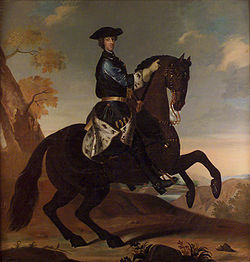
\includegraphics[height=0.5\textheight]{test_image}
\caption{En typisk rymdhiss enligt Wikipedia. Bildkälla (\cite{sampleitem1}).}
\label{fig:space}
\end{figure}

This report covers... \cite{sampleitem2}

\section{Introduction}

\subsection{Research Question}

This research question deals with the procedural generation of road networks from example data sets, and the edge cases that arise when dealing with footpath planning. A common problem is that footpaths are in their nature placed densely. How can the program identify critical areas where the footpath width is so large that it collides with existing roads? Can this be done so efficiently that the example-driven program can still run in real time? An additional question that arises is how much road data will be necessary to create believable procedural road networks for new zones in the Stockholm metropolitan area. How can this data be sampled and processed efficiently?

The previous work by Nishida et. al. has shown that it is possible to create believable procedural road maps from examples. Their program has created a network of 35 km road in less than a second, so for the application of zoning new city areas my hypothesis is that such a program can be made to run in real time with such minimal waiting time that it can be used in a real application by a city planner.

The challenge lies in how to extract the footpath data and tie it together with the existing road map. the work by Nishida et. al. only deals with arterial and secondary roads, and I will be adding a tertiary layer of roads, wich is highly possible, but may increase the data consumption and program running time. The same applies for the statistical model that identifies colliding roads, which I will be adding on top of that.

\subsection{Problem Constraints}

\begin{enumerate}
\item The road network is assumed to be a 2D simple graph. This means that any overlapping roads, such as tunnels and bridges that cross over street-level roads, will be eliminated from the training set. Any self-connected nodes will also be eliminated from the training set.
\item It will be assumed that the city map consists of only arterial (primary) roads, secondary roads and footpaths.
\item It will be assumed that the primary, secondary and tertiatry roads all have a fixed width. Primary roads have a set width, and secondary roads and footpaths as well.
\item It will be assumed that the use case of the application is for generating areas with the size of a neighbourhood or a few city blocks. The area that the user will sketch will typically be around 0.1 km2.
\item The program will not handle terrain features and altitude. It will be assume that the road mesh is projected on a flat 2D surface.
\end{enumerate}

With that said, Nishida et. al. present an excellent solution for generating new road patches that comform to an underlying terrain function.

\subsection{Evaluation}

The question will be examined primarily by creating a piece of software that can generate urban maps with primary and secondary roads, as well as footpaths, from example. I will experiment with different methods of collecting road data as well as different sample amounts and densities.

The evaluation plan will consist of programmatic evaluations and quantifyable metrics. My main idea is to sample metrics about intersections only (number of connecting roads, the angles between them, distance to connecting intersections, curviness of roads, etc). If I can sample all that and create a distribution for a few different cities, I have the two following hypothesises:
  1. There should be selection of features that produce an observable difference in the distributions between cities that look vastly different.
  2. If I let my program generate a large number of city parcels from a dataset, the resulting feature distribution should look like to the source dataset, and unlike datasets of other cities.
These distributions could be created for primary, secondary roads and footpaths separately.

\subsection{Background}

Procedural modeling of road networks is of interest to the fields of urban planning and urban architecture. In recent years there has been an advent of interactive tools that aid urban planners in placing or generating features of an urban plan, particularly roads and road networks.
Additionally, the topic is of interest for 3D content creators in for example the fields of video game design or 3D animation. A trend in these fields is using methods of procedural modeling to create large amounts of 3D content quickly and efficiently, while requiring as little hand modeling as possible. Studios who create large worlds are often interested in solutions that generate large road networks without any hand modeling.

Motivation

Navigation agents, they might fail navigating when faced with a too narrow path or intersecting obstacles
Using a road network to creates an underlying navmesh

\subsection{ESAL, KTH}
The thesis work will be carried out at the Embodied Social Agents Lab (ESAL) at the Department of Computational Science and Technology (CST). The lab has before been working on systems for generating procedural urban environments, and are interested in the possibility of generating more detailed maps than have been done before, using example-based methods to preserve the aesthetic look of a greater metropolitan area. The lab is particularly interested in the generation of footpaths, since most commercial software that import road maps only import arterial and secondary car roads, and do not include pedestrian walkways, cycle paths and such smaller roads.
% TODO: any official description of ESAL that can be used here?

\section{The geodata used in this project}

For the purpose of this project, the OpenStreetMap road dataset has been used in the presentation of the road network around Stockholm, and in the generative process of new road networks. To assess and correct path widths and path node locations, the OpenStreetMap building footprint dataset has also been used. To make an assessment on the quality and precision of the OpenStreetMap data, the SLU map from the Swedish National Land Survey was used in comparison with the OpenStreetMap map. The SLU map conatins only building footprints and property limits. Both map segments were obtained around the Stockholm greater metropolitan area. The exact map segments that were extracted were in both cases rectangles with the following coordinates:. TODO: Get coordinates

\subsection{OSM Data}

OpenStreetMap road data and building footprints are commonly obtained by manually tracing features in commercially available satellite images. Such images have a limit on their resolution which puts a theoretical limit on the accuracy of map features compared to their real-world equivalents (Haklay 2010). Particularily the high resolution imagery from Bing in 2010 led to an increase in building information in OpenStreetMap (Fan et al, 2014).

To separate sidewalks from detached footpaths, I used the fact that OSM generally provides sidewalks with the same name as the adjacent motorway. Thus they can be paired together and measured against each other.

\subsection{SLU Data}

The SLU map contains building features and property limits, but no road data.
The SLU map is maintained by The Swedish National Land Survey (Swedish: Lantmäteriet).
The SLU data is aqqcuired by land surveying methods such as GPS or DGNSS positioning, or by reproduction of features from ortophoto or stereo mapping from 3D aerial images.
The map is updated continously by Lantmäteriet, in conjoncture with the forming or reforming of property.
Property limits and building features have a position accuracy requirement of 5 meters.
(Lantmäteriet, 2019)

\subsection{A word on coordinate systems}

The SLU dataset is delivered in the SWEREF 99 TM (Lantmäteriet, 2019). SWEREF 99 TM is a projected coordinate system and there is no linear transformation to WGS 48, which OpenStreetMap uses (OSM 19). The coordinate conversions for this paper were obtained using proj: a Linux commandline application for geospatial coordinate conversion.

\section{Evaluation of the quality of geodata}

(Haklay 2010) specifices a comprehesive list of 8 accuracy classes when it comes to evaluating the quality of geographic information.

\begin{itemize}
  \item Lineage. This is the historical aspect of the dataset, which concerns the collection process and evolution.
  \item Positional accuracy. This relates the coordinate value of an object in the database to the actual location of the ground in the real world.
  \item Attibute accuracy. In a geographical database, objects are commonly tagged with meta-information. This class assesses how correct those values are.
  \item Logical consistency - This assesses the internal consistency of the dataset. For every dataset there may be internal rules and relationships that objects and features must follow, and this class assesses the degree to which these are adhered to.
  \item Completeness - This assesses the lack of data in a dataset, and the coverage of real-world objects. Objects or features may be missing from a dataset, which reduces its quality.
  \item Semantic accuracy - This links the way in which an object or feature is recorded and represented to how it should be interpreted.
  \item Usage, purpose and constraints - This concerns the validity of the dataset in relation to its purpose and how it is used.
  \item Temporal quality - This assesses the validity of the dataset in relation to real-world changes over time.
\end{itemize}

Other than for the purpose of mentioning various sources or error, this project will focus exclusively on the Positional accuracy, Completeness and Semantic accuracy classes. The comparison of the OSM and SLU maps will focus on these accuracy classes to determine the error tolerance when manipulating features in the 3D map presentation and the road network generating phase.

\subsection{The accuracy classes that will not be focused on}

The lineage aspect of the OSM data is available through the OSM History Viewer, an online debugging tool that lets anyone freely view the change history of individual fetures in a commit history-like fashion. There is an option for editors to include a personal note with their changesets to include additional details or motivate why a change was made, but there is no guaratee that the data includes any information on the aquisition method used (OSM 2020). The history aspect of the SLU dataset is not freely available online, but the acquistion method is included in the file metadata on a per-object basis. Lantmäteriet uses internal codes to specifify the acquistion method, and these codes can be referred to in the product description the accompanies the map files. As the scope of this project is limited to making a broad comparison of the positional accuracy of the two datasets, only the required positional accuracy as described by the SLU product description will be used.
TODO: Dig deeper in the SLU dataset, how can one find the method of aquisition for Stockholm buildings, and its precision?

The attribute accuracy measure is interesting, as both maps use encoded metadata on a per feature basis, the attribute accuracy of the two datasets could be assessed by doing a simple feature comparison and creating a translation table between the two attribute maps. To the knowledge of the author, this has never been done with specifically these two datasets, at the time of writing.

The temporal accuracy will not be assessed as this projects focuses on comparing a single snapshot of the two datasets at the same point in time.

The logical accuracy will not be assessed because the underlying logical relations between features in both maps serve no purpose to this project.

\section{Dataset quality evaluation}

\subsection{Assesment of dataset completeness}

(Fan et al., 2014) used the total building area in their reference dataset and the OpenStreetMap dataset to assess the completeness of OpenStreetMap data. The motivation for this is to eliminate semantic differences between both datasets. A very common example of a semantic error when comparing geographic data is that a large building in one dataset may be segmented into several smaller ones in the other, making one-to-one object mapping impossible. Thus using building area as an estimator for completeness solves this issue much better than i.e. the number of buildings or other objects in each dataset.
This project will use the building area in the OSM dataset versus that of the SLU dataset to determine the completeness of OpenStreetMap building data in the Stockholm area, which will then be used as an argument for how accurate the building correspondence and point proximity measures can be.

\subsection{Building correspondence}

Feature mapping
The building footprint correspondence will be evaluated using a similarity function that assesses the turning funciton and relative area overlap. The similarity function between any building in the OSM data set and any building in the SLU datasets will be defined as a function of their respective footprints ($foot_{OSM}, foot_{SLU}$), as follows:
$S(foot_{OSM}, foot_{SLU}) = S_{T}(foot_{OSM}, foot_{SLU}) + S_{RO}(foot_{OSM}, foot_{SLU})$, where $S_{T}$ measures the difference in turning function and $S_{RO}$ measures the relative overlap between the footprints.

\subsection{Turning function definition}

The turning function was first defined by Arkin et al. (1991), as a method for measuring the similarity of two polygons. The Turning function $T_c(l)$ measures the cumulative angle of the polygon's counter-clockwise tangent, as a function of the cumulative normalized length l. This project uses the turning function as it is defined by (Fan et al., 2014). For a polygon with vertices ${v_1 ... v_n}$ and line segments ${e_1 ... e_n}$ It is defined as follows.
Fix a starting vertex $v_1$.
The tangent angle at $v_1$ is $\theta_{n,1}$. This is the angle between the neighbouring line segments $e_n$ and $e_1$.
For any $i$ such that $i>1$ and $n<i$, the tangent angle at $v_i$ is recursively defined as: $\theta_{i, i-1} = \theta_{n,1} + \sum^{i}_{k=1} \theta_{k, k-1}$
The turning function has some nice geometric properties, in that it is invariant to both rotation and scaling of the polygon. The function contains no information of the orientation of the polygon, only of the relative angle between successive line segments, thus it does not change under roation. It also measures only the normalized cumulative length, which does not change under scaling.
The similarity of two polygons A and B in terms of their turning function is defined as their distance of their cumulative turning functions: $S_{T}(A, B) = 1 - (\int^{1}_{0} T_{C,A}(l) - T_{C,B}(l) dl)^{1/2}$.
The value range will be $(0 < S_{T} < 1)$, where $S_{T}(A,B) = 1$ if the polygons are identical. 

\subsection{Correspondence by building area}

(Fan et al., 2014) further discussed how the relative overlap in building area can be used to determine building correspondence between datasets, in cases where there is not much displacement between OSM building footprints data and the reference data set. Figure X (TODO) shows a typical comparison between the OpenStreetMap and SLU datasets, and by eyesight it was determined that the displacement of features is small. The relative building overlap between the OSM and SLU datasets will be defined as folows, given the footprints of any building in the OSM set ($foot_{OSM}$) and the SLU set ($foot_{SLU}$):

$S_{RO}(foot_{OSM}, foot_{SLU}) = \frac{A_{Overlap}}{min(A_{foot_{OSM}}, A_{foot_{SLU}}))}$

For this project the relative overlap will be used both to find possible matching building candidates, and as a term in their similarity function.

The relative overlap may be used to determine building matching relations even when the semantic accuracy is low. If a large building is represented by a single footprint in one dataset but by several smaller footprints in the other, (Rutzinger et al, 2009) found that if $S_{RO}(foot_{A}, foot_{B}) < 30\%$ for two buildings $A$ and $B$ from different sets, then $A$ and $B$ are highly likely to be separate, neighbouring buildings and not in fact identical. Therefore we will here assume that two buildings are matching candidates if their relative area overlap is greater than 30\%. If a one-to-many object matching is found, the compound perimeter of the footprints in the many-set will be used when calculating the turning function and finding closest vertices between the polygons.

\subsection{Closest point and point proximity}

The final problem is that even when building polygons have been matched between the two datasets, they may not have one-to-one vertex relationship. Footprints from different datasets may be formed at a different level of detail. Problems that arise are e.g. that the vertex counts are dissimilar, or that vertex clusters may be found at different parts of the polygon in the two datasets. To avoid this effect, key points are extracted using the Douglas-Peucker algorithm (Douglas and Peucker, 1973), to create a simplifed footprint with less points that still retain information about the rough features of the detailed footprint. The idea behind Douglas-Peucker is to recursively divide a polyline. It initially marks only the start and end points $(v_0, v_n)$ to be kept, and finds the point $v_i$ in between whose distance is the greatest to the line segment between $v_0$ and $v_n$. It then recursively refines the line segments $(v_0, v_i)$ and $(v_i, v_n)$, and proceeds to do so until a line segment $(v_j, v_k)$ is found, where every point in between $v_j$ and $v_k$ have a distance to the line segment $(v_j, v_k)$ that is smaller than some resolution $\epsilon$. Then $v_j$ are added to the simplified polyline, and all nodes in between them are discarded. See Algorithm 1 for a detailed view. In either case The minimum bounding rectangle (MBR) is calculated for the two polygons. Finally the MBR for the OSM building footprint is shifted so that its centroid aligns with the centroid of the MBR of the SLU building footprint. Any edges in the simplified footprints that coinside with the MBR from the same dataset are extracted, and the corresponding points in the original footprints will be matched with each other.

\begin{algorithm}[H]
\SetAlgoLined
\KwResult{Write here the result }
    // Find the point with the maximum distance\;
    $d_{max}$ = 0\;
    $index$ = 0\;
    $end$ = length(PointList)\;
    
    \For{$i$=2 to ($end$-1)}{
        $d$ = perpendicularDistance(PointList[$i$], Line(PointList[1], PointList[$end$]))\;
        \If{$d$ $>$ $d_{max}$} {
            $index$ = $i$\;
            $d_{max}$ = $d$\;
        }
    }

    ResultList = []\;
    
    // If max distance is greater than epsilon, recursively simplify\;
    \eIf{$d_{max}$ $>$ $\epsilon$} {
        // Recursive call\;
        recResults1[] = Douglas-Peucker(PointList[1...$index$], $\epsilon$)\;
        recResults2[] = Douglas-Peucker(PointList[$index$...$end$], $\epsilon$)\;

        // Build the result list\;
        ResultList[] = {recResults1[1...length(recResults1) - 1], recResults2[1...length(recResults2)]}\;
    }{
        ResultList[] = {PointList[1], PointList[$end$]}\;
    }
    \Return{ResultList[]}\;

    \caption{Douglas-Peucker}
\end{algorithm}

Finally, when two building footprints and their vertices have been mapped, we will use the offset of matching vertices as a measure of positional error. The average and variance in vertex spread will be calculated and used to make an assessment of the geometric precision of the OpenStreetMap dataset, and this precision will further be used to form an upper boundary on geometrical corrections that can be made to the map once it has been imported into the application.

\section{Implementation}

In this implementation, roads of different types were allowed to merge into one another to form common intersections. To facilitate this, it was neccessary to work with a path-by-path representation of the point data. When two path share a node with common coordinates, they form an intersection which can be of multiple different types.

\begin{thebibliography}{9}

\bibitem{lantmateriet-19}
(Lantmäteriet, 2019), Produktbeskrivning: GSD-Fastighetskartan vektor \\ 
\href{https://www.lantmateriet.se/globalassets/kartor-och-geografisk-information/kartor/fastshmi.pdf}.

\bibitem{osm-19}
(OSM 19) Converting to WGS84, accessed 13-03-2020 \\ 
\href{https://wiki.openstreetmap.org/wiki/Converting\_to\_WGS84}.

\bibitem{osm-20}
(OSM 20) OSM History Viewer\\
\href{https://wiki.openstreetmap.org/wiki/OSM\_History\_Viewer}.

\bibitem{haklay-10}
(Haklay, 2010), How good is volunteered geographical information?A comparative study of OpenStreetMap and OrdnanceSurvey datasets \\
\href{https://kfrichter.org/crowdsourcing-material/day1/haklay10.pdf}.

\bibitem{fan-14}
(Fan et al, 2014), Quality assessment for building footprints data on OpenStreetMap \\
\href{https://www.researchgate.net/publication/262163378\_Quality\_assessment\_for\_building\_footprints\_data\_on\_OpenStreetMap}.

\bibitem{arkin-91}
Arkin E.M., Chew L.P., Huttenlocher D.P., Kedem K. and Mitchell J.S.B. 1991. An Efficiently Computable \\
Metric for Comparing Polygonal Shapes. In: IEEE Transaction on Pattern Analysis and Machine \\
Intelligence, Vol. 13, No. 3, March 1991. \\

\bibitem{douglas-peucker-73}
Douglas, D.H. and Peucker T.K. 1973. Algorithms for the reduction of the number of points required to \\
represent a digitalized line or its caricature. In: Cartographica: The International Journal for Geographic \\
Information and Geovisualization, 10(2), 112-122. \\

\bibitem{rutzinger-09}
Rutzinger, M., Rottensteiner, F. and Pfeifer, N. 2009. A Comparison of Evaluation Techniques for Building \\
Extraction From Airborne Laser Scanning. IEEE Journal of Selected Topics in Applied Earth \\
Observations and Remote Sensing 2(1): 11-20. \\

\end{thebibliography}


\end{document}
